\documentclass[9pt]{beamer}

% \usepackage[T1]{fontenc}
\usepackage[utf8]{inputenc}
\usepackage[russian]{babel}
\usepackage{graphicx}
\usepackage{hyperref}
\graphicspath{ {images/} }

\usetheme{Goettingen}


\title{Использование сонаров для решения задачи картографирования в мобильной робототехнике}

% A subtitle is optional and this may be deleted
% \subtitle{Optional Subtitle}

% \author{Денис Шепелев\inst{1}}
\author{Денис Шепелев}

% - Give the names in the same order as the appear in the paper.
% - Use the \inst{?} command only if the authors have different
%   affiliation.

\institute[Universities of Somewhere and Elsewhere] % (optional, but mostly needed)
{
  % \inst{1}%
  % 073а\\
  ИППИ РАН \\ МФТИ
}
% - Use the \inst command only if there are several affiliations.
% - Keep it simple, no one is interested in your street address.

\date{58 научная конференция МФТИ, 2015}
% \date{}

\begin{document}

\begin{frame}
  \titlepage
\end{frame}

% \begin{frame}{Outline}
%   \tableofcontents
%   % You might wish to add the option [pausesections]
% \end{frame}

% Section and subsections will appear in the presentation overview
% and table of contents.


% \begin{frame}{Name}
% \begin{columns}
%   \begin{column}{0.50\textwidth}
%     \begin{itemize}
%       \item
%       {
          
%       }
%     \end{itemize}
%   \end{column}
%   \begin{column}{0.50\textwidth}
%     \begin{figure}[h]
%       \centering
%       \includegraphics[width=0.8\textwidth]{name.png}
%     \end{figure}
%   \end{column}
% \end{columns}

% \end{frame}

\section{2D карты и датчики}

\subsection{2D карта}

\begin{frame}{2D карта}
\begin{columns}
  \begin{column}{0.50\textwidth}
    \begin{itemize}
      \item
      {
        Карта - обычное изображение
      }
      \item
      {
        Каждый пиксель - некоторая область пространства
      }
      \item
      {
        Белый пиксель - свободная для движения область
      }
      \item
      {
        Черный - чем-то занятая облать
      }
      \item
      {
        Серый - неизвестная область
      }
    \end{itemize}
  \end{column}
  \begin{column}{0.50\textwidth}
    \begin{figure}[h]
      \centering
      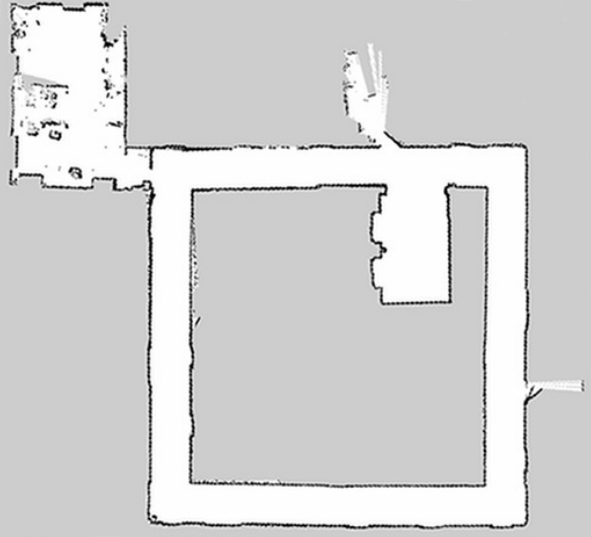
\includegraphics[width=0.8\textwidth]{grid_map.png}
    \end{figure}
  \end{column}
\end{columns}
\end{frame}

\subsection{Датчики}

\begin{frame}{Датчики}

\begin{itemize}
  \item
  {
    Сонары
  }
  \item
  {
    Лидары
  }
  \item
  {
    Стереокамеры
  }
\end{itemize}

\end{frame}

\subsection{Задача 2D картографирования}

\begin{frame}{Задача 2D картографирования}
\textbf{Дано}:
\begin{itemize}

  \item
  {
    Есть данные датчиков
  }
  \item
  {
    Известно положение робота, в любой момент времени
  }
  \item
  {
    Окружение статично
  }
\end{itemize}
\textbf{Цель}:
\begin{itemize}
  \item
  {
    Построить карту с учетом вышесказанного
  }
\end{itemize}
\end{frame}

\begin{frame}{Датчики}

\begin{itemize}
  \item
  {
    Сонары.
    \begin{itemize}
    \item
    {
      Достаточно точны для широкого круга задач
    }
    \item
    {
      Отностительно дешевые
    }
    \end{itemize}
  }
  \item
  {
    \textcolor{red}{Лидары}
  }
  \item
  {
    \textcolor{red}{Стереокамеры}
  }
\end{itemize}

\end{frame}

\section{Подходы к решению задачи}

\subsection{Подходы к решению задачи}

\begin{frame}{Подходы к решению задачи}
Различают два основных подхода к решению задачи 2D картографирования:
\begin{itemize}
  \item
  {
    с обратной моделью сенсора

    $$P(m|z)$$
  }
  \item
  {
    с прямой моделью сенсора

    $$P(z|m)$$
  }
\end{itemize}

\end{frame}

\subsection{Алгоритм с обратной моделью сенсора}

\begin{frame}{Алгоритм с обратной моделью сенсора}

\begin{itemize}
  \item
  {
    Итеративный алгоритм, работает в режиме реального времени
  }
  \item
  {
    Клетки - назависимые случайные величины
  }
  \item
  {
    В каждой клетке хранится вероятность того, что она занята.
  }
  \item
  {
    Значения в клетках обновляются по формуле

    \begin{equation}
      \begin{split}
        \frac{P(m_i | z_{1:t}, x_{1:t})}{1 - P(m_i | z_{1:t}, x_{1:t})} = 
        \frac{P(m_i | z_t, x_t)}{1- P(m_i | z_t, x_t)}\\
        \frac{P(m_i | z_{1..t-1}, x_{1:t-1})}{1- P(m_i | z_{1..t-1}, x_{1:t-1})}\\
        \frac{1 - P(m_i)}{P(m_{i})}
      \end{split}
    \end{equation}
  }
\end{itemize}
\end{frame}

\begin{frame}{Алгоритм с обратной моделью сенсора}

\begin{itemize}
  \item
  {
    Отлично подходит для лидаров
  }
  \item
  {
    Не подходит для работы с сонарами
  }
\end{itemize}
\end{frame}


\begin{frame}{Алгоритм с обратной моделью сенсора}
При получении формулы (1) предполагается, что
$P(z_t|m_{ij}, z_{1:t-1}) = P(z_t|m_{ij})$ - для сонаров плохое допущение

\begin{columns}
\begin{column}{0.33\textwidth}
  \begin{figure}[h]
    \centering
    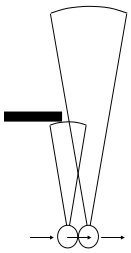
\includegraphics[width=0.65\textwidth]{inv1.png}
  \end{figure}
\end{column}
\begin{column}{0.33\textwidth}
\begin{figure}[h]
    \centering
    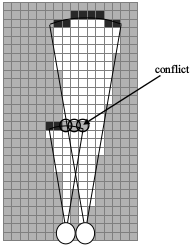
\includegraphics[width=0.9\textwidth]{inv2.png}
\end{figure}
\end{column}
\begin{column}{0.33\textwidth}
  \begin{figure}[h]
    \centering
    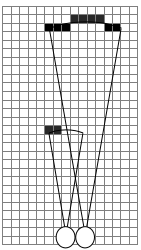
\includegraphics[width=0.7\textwidth]{inv3.png}
  \end{figure}
\end{column}
\end{columns}
\end{frame}

\begin{frame}{Алгоритм с обратной моделью сенсора}
\begin{figure}[h]
    \centering
    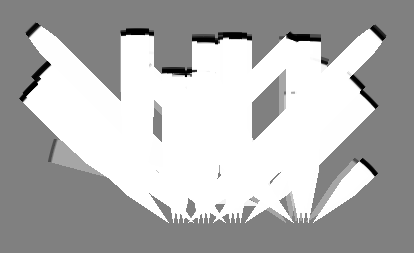
\includegraphics[width=0.7\textwidth]{inv_ex.png}
  \end{figure}
\end{frame}

\subsection{Алгоритм с прямой моделью сенсора}
\begin{frame}{Алгоритм с прямой моделью сенсора}
\begin{itemize}
  \item
  {
    В каждом пикселе хранится либо 1, либо 0. 
  }
  \item
  {
    Вместо обратной модели использовать прямую модель $P(z|m)$
  }
  \item
  {
    Накопления данных с сонаров
  }
  \item
  {
    Максимизация правдоподобия $P(z|m)$ перебирая карты $m$
  }
  \item
  {
    Прямая реализация алгоритма не подразумевает работу в режиме реального времени
  }
\end{itemize}
\end{frame}

\subsection{Итеративный алгоритм с прямой моделью сенсора}

\begin{frame}{Итеративный алгоритм с прямой моделью сенсора}
Пусть есть некоторая карта $m$ и список наблюдений сонаров $z$, тогда:
\begin{itemize}
  \item
  {
    Реальное окружение таково, что большинство клеток будут свободными, поэтому штрафуем все черные клетки на величину $-p_{free}$. Таким образом значение функцинала $$\phi_{free}(m^{k}) = \sum_{x \in m: x=1}{-p_{free}}$$
  }
\end{itemize}
\end{frame}

\begin{frame}{Итеративный алгоритм с прямой моделью сенсора}
\begin{itemize}
  \item
  {
    Также для каждой клетки вводится величина согласованности с соседями. Например, естественно считать что, если большинство соседей заняты, то и рассматриваемая клетка, скорее всего, занята. Поэтому за каждого соседа согласующегося с клеткой прибавляем $p_{a}$, иначе вычитаем $p_a$

    Пример:

    \begin{figure}[h]
      \centering
      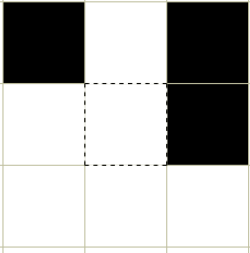
\includegraphics[width=0.25\textwidth]{cells.png}
    \end{figure}

    Клетка белая, тогда $\phi_a(m_{ij}) = 5p_a - 3p_a = 2p_a$

    $$\phi_a(m) = \sum_{m_{ij}} \phi_a(m_{ij})$$
  }

\end{itemize}

\end{frame}


\begin{frame}{Итеративный алгоритм с прямой моделью сенсора}
\begin{itemize}
  \item
  {
    Используя список $z$ данных сонаров, обновляем значение  $$\phi_{z}(m) = \sum_{s=1}^l \log{P(z_s|m)}$$ 
  }
  \item
  {
    Таким образом задача картографирования сводится к максимизации величины $$\Phi(m, z) = \phi_{free}(m) + \phi_a(m) + \phi_{z}(m) $$
  }
  
\end{itemize}
\end{frame}


\begin{frame}{Итеративный алгоритм с прямой моделью сенсора}
\begin{itemize}
  \item
  {
    При k = 0: считаем значения 
    $$\phi_{free}(m^{0}), \phi_a(m^{0}), \phi_{z}(m^{0})$$ 
    $$\Phi(m^{0}, z) = \phi_{free}(m^{0}) + \phi_a(m^{0}) + \phi_{z}(m^{0})$$
    $$m = m^0$$
    $$\Phi(m, z) = \Phi(m^{0}, z)$$
  }
  \end{itemize}
\end{frame}

\begin{frame}{Итеративный алгоритм с прямой моделью сенсора}
\begin{itemize}
  \item
  {
    На шаге $k$ получаем карту $m^{k}$ из $m^{k-1}$ меняя значение случайной клетки ${ij}$ на противоположное. Затем:
    \begin{enumerate}
      \item
      {
        Если пиксель стал свободным $\phi_{free}(m^{k}) = \phi_{free}(m^{k}) + p_{free}$,\\ иначе $\phi_{free}(m^{k}) = \phi_{free}(m^{k}) - p_{free}$
      }
      \item
      {
        Для клетки считаем значение величины согласованности $\phi_a(m_{ij})$
        $$\phi_a(m^k) = \phi_a(m^{k-1}) - (8p_a - 2\phi_a(m_{ij}))$$
      }
      \item
      {
        Используя текущий список из последних $l$ данных сонаров $z$,  обновляем значение функционала $$\psi_{z}(m^{k}) = \sum_{s=1}^l \log{P(z_s|m^k)}$$
      }
      \item
      {
        Пересчитываем $\Phi(m^{k}, z)$. 
        Если $\Phi(m^{k}, z) > \Phi(m, z)$ или рандом:
        $$\Phi(m, z) = \Phi(m^{k}, z), m = m^k$$
        иначе
        $$\Phi(m^{k}, z) = \Phi(m, z), m^k = m $$
      }
    \end{enumerate}
  }
  \end{itemize}
\end{frame}


\subsection{Прямая модель сонара}

\begin{frame}{Прямая модель сонара}
\begin{itemize}
  \item
  {
    Пусть есть занятая клетка $\{ij\}$
  }
  \item
  {
    $p(z|m_{ij})$ - величина, которая характеризует степень согласования состояния клетки с наблюдением сонара z 
  }
  \item
  {
    Например $p(z|m_{ij})$ - гауссово распределение от угла между сонаром и точкой $\{ij\}$ и расстояния, измеренного сонаром.
  }
\end{itemize}
\end{frame}

\begin{frame}{Прямая модель сонара}
\begin{itemize}
  \item
  {
    У сонара есть некоторая область видимости. Ясно, что те клетки, которые не лежат в области видимости датчика, никак не влияют на $p(z|m)$
  }
  \item
  {
    $p(z|m) = p(z|m_{in})$, где $m_{in} = \{ m_1, ..., m_K\}$ - отсортированное по расстоянию от сенсора множество клеток в области видимости сонара.
  }
  \item
  {
    $$p(z|m_{in}) = \sum_{k=1}^K{q (1-q)^k p(z|m_{k})}$$
    $q$ - вероятность того, что измерение $z$ стало результатом отражения звуковой волны от клетки $m_{ij}$
  }
\end{itemize}
\end{frame}



\section{Результаты и дальнейшие планы}
\begin{frame}{Результаты}
\begin{columns}
\begin{column}{0.5\textwidth}
  
  \begin{figure}[h]
    \centering
    
\includegraphics[width=0.9\textwidth]{inv_line_ex.png}
  \end{figure}

\end{column}
\begin{column}{0.5\textwidth}
  \begin{figure}[h]
    \centering
    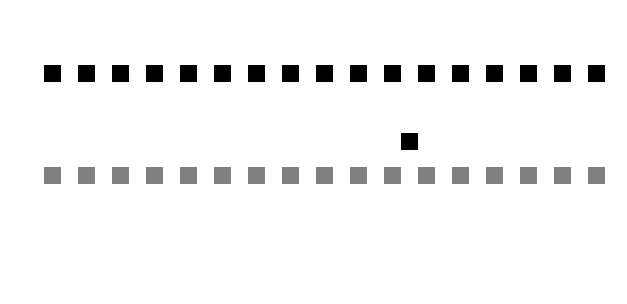
\includegraphics[width=0.9\textwidth]{line_ex.png}
  \end{figure}
\end{column}
\end{columns}
\end{frame}

\begin{frame}{Результаты}
\begin{columns}
\begin{column}{0.5\textwidth}
  
  \begin{figure}[h]
    \centering
    
\includegraphics[width=0.9\textwidth]{inv_arc_ex.png}
  \end{figure}

\end{column}
\begin{column}{0.5\textwidth}
  \begin{figure}[h]
    \centering
    
\includegraphics[width=0.9\textwidth]{arc_ex.png}
  \end{figure}
\end{column}
\end{columns}
\end{frame}

\begin{frame}{Результаты}
\begin{columns}
\begin{column}{0.5\textwidth}
  
  \begin{figure}[h]
    \centering
    
\includegraphics[width=0.9\textwidth]{inv_room_ex.png}
  \end{figure}

\end{column}
\begin{column}{0.5\textwidth}
  \begin{figure}[h]
    \centering
    
\includegraphics[width=0.9\textwidth]{room_ex.png}
  \end{figure}
\end{column}
\end{columns}
\end{frame}

\begin{frame}{Результаты и дальнейшие планы}
Результаты
\begin{itemize}
  \item
  {
    Реализован алгоритм с обратной моделью сонара
  }
  \item
  {
    Разработан и реализован алгоритм с прямой моделью, который (пока) использует все накопленные данные сонаров
  }
  \item
  {
    Скрипты для создания исскуственных данных для тестирования
  }
\end{itemize}
Планы
\begin{itemize}
  
  \item
  {
    Поиск оптимальных параметров алгоритма с прямой моделью
  }
  \item
  {
    Дальнейшее улучшение прямой модели
  }
  \item
  {
    Сбор и тестирование на реальных/сгенерированных данных
  }
  \item
  {
    Разобраться с проблемой забывчивости карты
  }
  \item
  {
    ...
  }
\end{itemize}
\end{frame}

% \begin{frame}{Name}
% \begin{itemize}
%   \item
%   {
      
%   }
% \end{itemize}
% \end{frame}


% All of the following is optional and typically not needed. 
\appendix
\section<presentation>*{\appendixname}
\subsection<presentation>*{Источники}

\begin{frame}[allowframebreaks]
  \frametitle<presentation>{Источники}
    
  \begin{thebibliography}{10}
    
  \beamertemplatebookbibitems
  % Start with overview books.

  \bibitem{ LL }
    Thrun S. [at al.]
    \newblock {Probabilistic robotics.}
    \newblock {\em Cambridge: MIT, 2005. – 672 с.}

  %   \newblock {\em Материалы лекции Фрайбургского университета по курсу Introduction to
  %   Mobile Robotics - Techniques for 3D Mapping}.
 
  \beamertemplatearticlebibitems
  % Followed by interesting articles. Keep the list short. 

  \bibitem{thr}
    Thrun S.
    \newblock {Learning Occupancy Grid Maps with Forward Sensor Models.}
    \newblock {\em Autonomous Robots. – 2003. – V. 15, I. 2. – p. 111-127.}

  \bibitem{Elfes}
    A. Elfes  
    \newblock {Occupancy Grids: A Stochastic Spatial Representation for Active Robot Perception.}
    \newblock {\em arXiv preprint arXiv:1304.1098. – 2013.}

  \end{thebibliography}
\end{frame}

\end{document}


